\documentclass[a4paper,12pt]{article} % This defines the style of your paper

\usepackage[top = 2.5cm, bottom = 2.5cm, left = 2.5cm, right = 2.5cm]{geometry}

\usepackage[T1]{fontenc}
\usepackage[utf8]{inputenc}

\usepackage{multirow} % Multirow is for tables with multiple rows within one cell.
\usepackage{booktabs} % For even nicer tables.

\usepackage{graphicx}
\usepackage{tikz}
\usepackage{xcolor}

\usepackage{setspace}
\setlength{\parindent}{0in}

\usepackage{float}

\usepackage{fancyhdr}


\pagestyle{fancy} % With this command we can customize the header style.

\fancyhf{} % This makes sure we do not have other information in our header or footer.

\rhead{splay\_experiment \hfill Jiří Klepl}

\cfoot{\footnotesize \thepage}

\begin{document}

\thispagestyle{empty} % This command disables the header on the first page.

\begin{center}
	{\Large \bf Homework 6 - matrix\_experiment}
	\vspace{2mm}

	{\bf Jiří Klepl}

\end{center}

\vspace{0.4cm}


\setlength{\parindent}{2em}

\section*{Prolog}

V následujících simulacích, čtyř simulovaných a jedné reálné, porovnáváme naivní implementaci (algoritmu ``řádek po řádku'') a cache-oblivious implementaci transponování čtvercové matice. Uvažovaná cache-oblivious implementace bude varianta algoritmu popisovaného na přednášce používající dvě subrutiny ($T$ a $TS$). Sledovaným parametrem je průměrný počet cache-miss na přístup a jeho závislost na velikosti oné matice. Obě implementace provádějí shodné změny na zadané matici, ale v jiném pořadí. Při simulacích je uvažována jednovrstvá cache s LRU strategií.

\section*{Simulované testy}

Jak bylo výše zmíněno, předpokládáme jednovrstvou cache s LRU strategií. Její velikost bude vždy udána parametrem $M$, velikost paměťových bloků (cache-line) potom parametrem $B$. Jeden experiment sestává z měření počtu cache-miss nad maticemi s rozměry $N \times N$, kde $N = 2^{\frac{i}{4}}; i \in \{20, 21, \dots 52\}$, vždy se stejnou cachí.

\subsection*{Vedlejší efekty na výsledky}

Pro všechny simulace platí, že optimalizér kódu nehraje žádnou roli (nemusí totiž tomu tak být u reálných experimentů) a že testovaný kód dokonale popisuje uvažované výpočty.

Na druhou stranu, reálným vliv na výsledky má její příprava. Ta je prováděna metodou ``řádek po řádku'' a jejím efektem je uložení posledních několika bloků do simulované cache. U velkých matic (ve srovnání k velikosti cache) to nebude mít významný vliv, ale u malých matic to bude potenciálně znamenat snížený počet cache-miss a u analýzy výsledků by toto mělo být zohledněno. Zejména pokud se matice celé vejde do cache, nastanou falešně nulové výsledky.

Výše zmíněný efekt může být v reálných aplikacích využit pro optimalizace, ale stojí na domluvě mezi jednotlivými algoritmy (kde na dané matici začínají a končí) a tedy není předmětem naší analýzy.

Velmi podobný efekt vznikne, když je matice moc malá na to, aby strategie swappování měly dostatečný vliv na počet cache-miss, například, když se celá matice vejde do cache.

\subsection*{Očekávané výsledky}

\subsubsection*{Odhad naivní implementace}

Pro všechny simulace bude očekávaný počet cache-miss na přístup u naivní implementace pracující nad dostatečně velkými maticemi přibližně roven $0.5$ (po krátkém vysvětlení uvedeme přesnější odhad). Toto pro nás bude sloužit jako horní limit, kterého lze jistě dosáhnout.

To plyne z toho, že při swapu je vždy jeden prvek pravděpodobně ve stejném bloku jako jeden z naposledy swappovaných prvků ($P_1 = \frac{1}{B}$), zatímco s ním swapovaný (s prohozenými souřadnicemi) je vždy v nenacachovaném bloku ($P_2 = 1$). Obojí dohromady má za výsledek průměrný počet cache-miss na přístup $P_{max} = \frac{B + 1}{2B} = 0.5 + \frac{1}{2B} \approx 0.5$.

\subsubsection*{Dolní mez cache-miss}

Dolní hranice průměrného počtu cache-miss je rovna $\frac{1}{B}$. To jde ukázat tím, že je nutno načíst $\frac{N^2}{B}$ bloků paměti za $N^2$ přístupů, tedy minimální průměrný počet cache-miss na přístup je $P_{min} = \frac{\frac{N^2}{B}}{N^2} = \frac{1}{B}$. Dosažení tohoto limitu je možné, pokud jsou algoritmem práce na paměťových blocích dokonale spárovány (například, konkrétně v použitém algoritmu, se v nějaké hloubce matice rozdělí na zrcadlové dvojice podmatic (samozřejmě podle diagonály), kdy tyto dvojice dokonale pokryjí cache; lze jednoduše zobecnit).

\subsubsection*{Horní odhad ideálního případu cache-oblivious implementace}

Horní odhad průměrného počtu cache-miss v ideálním případě je rovna $\frac{1}{B}$, je-li $2 B^2 \leq M$. Tedy, je-li cache po cache-line rozdělitelná na alespoň dva čtverce (tomu pak odpovídají zrcadlové dvojice podmatic, při počtu dělitelným čtyřmi virtuálně zdvojnásobíme cache-line), poté lze dosáhnout postupu popsaného výše. V opačném případě nalezneme mocninu dvou $B'$ takovou, že $2 B B' = M$, poté je horním odhadem ideálního případu $\frac{1}{B'} = \frac{2B}{M}$ a to odpovídá strategii, podobné minule diskutované, kdy však toto rozdělení tvoří použe podmnožina cache o velikosti $2 B'^2$, zbytek neužitečný, až na náhodné zlepšení.

\subsubsection*{Horní mez neideálního případu cache-oblivious implementace}

Nejprve budeme uvažovat ``polo-ideální'' případ. U libovolné dvojice podmatic z ideálního případu, kdy matice měly rozměry shodné s paměťovými bloky, když myšleně posuneme bloky paměti přesně o polovinu a rozdělíme zmíněné podmatice, každou na čtyři další, každou teď prochází $\frac{2B}{4} = \frac{B}{2}$ unikátních paměťových bloků a danou dvojicí tedy vždy $B$, tedy stejně, jako tomu bylo u původních podmatic v ideálním případě, tedy na celou dvojici podmatic je potřeba $4B$ načtení namísto $2B$. A toto lze dobře rozdělit LRU strategií cache.

Toto lze zobecnit pro libovolné posunutí bloků, kdy sousední dvojicí nových podmatic prochází maximálně $\frac{3B}{2}$ paměťových bloků, tedy na celou původní podmatici $3B$ a na dvojici tedy $6B$, to by nám dalo teoreticky trojnásobek ideálního odhadu, pokud stále zafunguje LRU strategie. Odpovědí je samozřejmě, že LRU strategie zafunguje a tohoto odhadu dosáhne téměř pouze, když je algoritmus dělen do podmatic v zašroubovávacím pořadí.

\subsubsection*{Počet cache-miss cache-oblivious algoritmu}

Průměrný počet cache-miss bude vždy v $\Theta\left(\frac{1}{B}\right) \cup \Theta\left(\frac{B}{M}\right)$.

\pagebreak

\subsection*{$M = 1024$ a $B = 16$}

\begin{figure}
	\caption{$M = 1024, B = 16$}
	\label{m1024b16}
	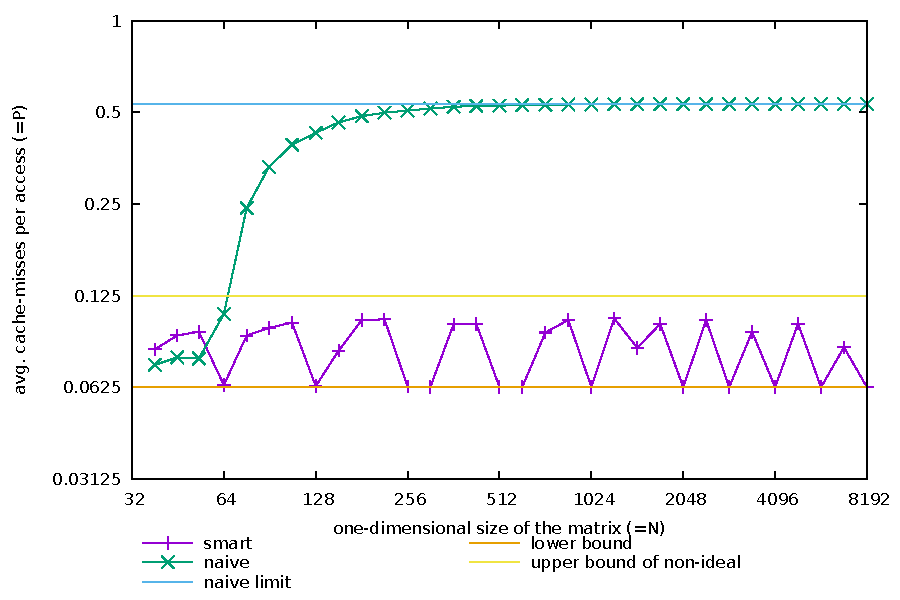
\includegraphics{sim-m1024-b16.pdf}
\end{figure}



\end{document}
